\documentclass{article}
\usepackage{amsmath}
\usepackage{amssymb}
\usepackage{graphicx}
\begin{document}
\section{Set Theory}
\begin{enumerate}
\item The Universal Set $\mathcal{U}$
\item Union
\item Intersection
\item Set Difference
\item Relative Difference
\end{enumerate}


%---------------------------------------%
\newpage

Question 2B 2010 Zone A


\begin{itemize}
	\item Let A and B be subsets of the a universal set $U$.
	\item Use membership tables to prove that $(A \cup B^{\prime})^{\prime}$ = $A^{\prime} \cap B$
	\item Shade the regions corresponding to this set on a Venn Diagram
\end{itemize}

\begin{array}{|c|c|| c | c| c|}
	A	&	B	&	$B^{\prime}$	&	$A \cup B^{\prime}$	&	$(A \cup B^{\prime})^{\prime}$	\\ \hline
	0	&	0	&	1	&	1	&	0	\\
	0	&	1	&	0	&	0	&	1	\\
	1	&	0	&	1	&	1	&	0	\\
	1	&	1	&	0	&	1	&	0	\\
\end{array}									


\begin{array}{|c|c|| c | c| }									
	A	&	B	&	$A^{\prime}$	&	$A^{\prime} \cap B$	\\	\hline	
	0	&	0	&	1	&	0	\\		
	0	&	1	&	1	&	1	\\		
	1	&	0	&	0	&	0	\\		
	1	&	1	&	0	&	0	\\		
\end{array}



%-------------------------------------------%
% 2010 Zone A Q 1c
Given the universal set $U$ and subsets $A$ and $B$, list the set $(A \cup B^{\prime})^{\prime}$
\begin{itemize}
	\item $U=\{1,2,\ldots,8,9\}$
	\item $A=\{2,4,6,8\}$
	\item $B=\{ 4,5,6,7\}$
	\item $B^{\prime}=\{ 1, 2, 3, 8, 9  \}$
	\item $A \cup B^{\prime}=\{ 1, 2, 3,4, 6, 8, 9  \}$
	\item $(A \cup B^{\prime})^{\prime}=\{ 5,7 \}$
\end{itemize}

%------------------------------------------$
2010 Zone B Q 1

5n+1 Rules of Inclusion method

$A = \{5n+1: n \in Z \}$
\subsection*{Floating Point Notation}
(Demonstration on white board)

\subsection*{2011 Zone A question 1d}

Showing your workings, express the repeating decimal 0.012012012012...
as a rational number in its simplest form.


\begin{itemize}
\item x = 0.012012012012...
\item 10x = 0.12012012012... (not particularly useful )
\item 100x = 1.2012012012... (not particularly useful either)
\item 1000x= 12.012012012... (very useful)
\item 999x = 12
\item x= 12/999 = 4/333 (Answer!)
\end{itemize}

%------------------------------------------$

\subsection*{2008  Zone A question2a}
$B = \{3n-1 :n \in Z^{+} \}$
Describe the set B using the listing method

\begin{itemize}
	\item Let $n=1$. Consequently $3(1)-1 =2$
	\item Let $n=2$. Likewise $3(2)-1 =5$
	\item Let $n=3$. $3(3)-1 = 8 $
	\item The repeated differences are 3. The next few values are 11, 14 and 17
	\item So by the listing method $B= \{2,5,8,11,14,17,\ldots\}$
\end{itemize}

$A = \{3,5,7,9,ldots \}$
Describe the set A using the rules of inclusion method

\begin{itemize}
	\item The repeated differences are 2.
	\item We can say the rule has the form $2n+k$
	\item For the first value n=1. Therefore $2+k=3$
	\item Checking this , for the second value , n=2. Therefore $4+k=5$
	\item Clearly k = 1.
	\item $A = \{2n+1 :n \in Z^{+} \}$
	\item So by the listing method $B= \{2,5,8,11,14,17,\ldots\}$
\end{itemize}

\section{Set Theory}
\begin{enumerate}
	\item The Universal Set $\mathcal{U}$
	\item Union
	\item Intersection
	\item Set Difference
	\item Relative Difference
\end{enumerate}

\newpage
%---------------------------------------%
\subsection*{Dice Rolls}
Consider rolls of a die. What is the universal set?

\[ \mathcal{U} = \{1,2,3,4,5,6\} \]

%--------------------------------------%
\subsection*{Worked Example}

Suppose that the Universal Set $\mathcal{U}$ is the set of integers from 1 to 9.
\[ \mathcal{U} = \{1,2,3,4,5,6,7,8,9\}, \]

and that the set $\mathcal{A}$ contains the prime numbers between 1 to 9 inclusive.

\[ \mathcal{A} = \{1,2,3,5,7\}, \]

and that the set $\mathcal{B}$ contains the even numbers between 1 to 9 inclusive.

\[ \mathcal{B} = \{2,4,6,8\}. \]

%--------------------------------------------------------%
\subsubsection*{Complements}
\begin{itemize}
	
	\item The Complements of A and B are the elements of the universal set not contained in A and B.
	
	\item The complements are denoted $\mathcal{A}^{\prime}$ and $\mathcal{B}^{\prime}$
	\[ \mathcal{A}^{\prime} = \{4,6,8,9\}, \]
	\[ \mathcal{B}^{\prime} = \{1,3,5,7,9\}, \]
	
\end{itemize}


%--------------------------------------------------------%

\subsubsection*{Intersection}
\begin{itemize}
	
	\item Intersection of two sets describes the elements that are members of both the specified Sets
	
	\item The intersection is denoted $\mathcal{A\cap B}$ 
	\[ \mathcal{A\cap B} = \{2\}\]
	
	\item only one element is a member of both A and B.
\end{itemize}
%--------------------------------------------------------%

\subsubsection*{Set Difference}
\begin{itemize}
	
	\item The Set Difference of A with regard to B are list of elements of A not contained by B.
	
	\item The complements are denoted $\mathcal{A-B}$ and $\mathcal{B-A}$
	\[ \mathcal{A-B} = \{1,3,5,7\}, \]
	
	\[ \mathcal{B-A} = \{4,6,8\}, \]
\end{itemize}
\subsection*{symbols}
$\varnothing$,
$\forall$,
$\in$,
$\notin$,
$\cup$
%----------------------------------------------------------- %
\newpage

\section*{Prepositional Logic}


%-------------------------------------------------------------- %
\begin{itemize}
	\item $p \wedge q$
	\item $p \vee q$
	\item $p \rightarrow q$
\end{itemize}
\newpage
\section{Sequence and Series and Proof by Induction}


\[\sum (n^2) \]

%--------------------------------------------------------%
\subsubsection*{Relative Difference}
\begin{itemize}
	\item $ A \otimes B$
\end{itemize}
%--------------------------------------------------------%
\subsubsection*{Power Sets}
\begin{itemize}
	\item Consider the set A where $ A = \{w,x,y,z\}$
	\item There are 4 elements in set A.
	\item The power set of A contains 16 element data sets.
	\item \[  \mathcal{P}(A) = \{\{ x \}, \{ y \} \}  \]
	\item (i.e. 1 null set, 4 single element sets, 6 two -elemnts sets, 4 three lement set and one 4- element set.)
\end{itemize}
%------------------------------------------------%
\newpage
\begin{itemize}
	\item $ p \rightarrow q$  p implies q
	\item $p \lg q $
\end{itemize}
\newpage

%--------------------------------------------------------%
\subsubsection*{Relative Difference}
\begin{itemize}
	\item $ A \otimes B$
\end{itemize}
%--------------------------------------------------------%
\subsubsection*{Power Sets}
\begin{itemize}
	\item Consider the set A where $ A = \{w,x,y,z\}$
	\item There are 4 elements in set A.
	\item The power set of A contains 16 element data sets.
	\item \[  \mathcal{P}(A) = \{\{ x \}, \{ y \} \}  \]
	\item (i.e. 1 null set, 4 single element sets, 6 two -elemnts sets, 4 three lement set and one 4- element set.)
\end{itemize}
%------------------------------------------------%
\newpage
\begin{itemize}
	\item $ p \rightarrow q$  p implies q
	\item $p \lg q $
\end{itemize}
%---------------------------- %
%---------------------------------------%
\subsection*{Dice Rolls}
Consider rolls of a die. What is the universal set?

\[ \mathcal{U} = \{1,2,3,4,5,6\} \]

%--------------------------------------%
\subsection*{Worked Example}

Suppose that the Universal Set $\mathcal{U}$ is the set of integers from 1 to 9.
\[ \mathcal{U} = \{1,2,3,4,5,6,7,8,9\}, \]

and that the set $\mathcal{A}$ contains the prime numbers between 1 to 9 inclusive.

\[ \mathcal{A} = \{1,2,3,5,7\}, \]

and that the set $\mathcal{B}$ contains the even numbers between 1 to 9 inclusive.

\[ \mathcal{B} = \{2,4,6,8\}. \]

%--------------------------------------------------------%
\subsubsection*{Complements}
\begin{itemize}

\item The Complements of A and B are the elements of the universal set not contained in A and B.

\item The complements are denoted $\mathcal{A}^{\prime}$ and $\mathcal{B}^{\prime}$
\[ \mathcal{A}^{\prime} = \{4,6,8,9\}, \]
\[ \mathcal{B}^{\prime} = \{1,3,5,7,9\}, \]

\end{itemize}


%--------------------------------------------------------%

\subsubsection*{Intersection}
\begin{itemize}

\item Intersection of two sets describes the elements that are members of both the specified Sets

\item The intersection is denoted $\mathcal{A\cap B}$ 
\[ \mathcal{A\cap B} = \{2\}\]

\item only one element is a member of both A and B.
\end{itemize}
%--------------------------------------------------------%

\subsubsection*{Set Difference}
\begin{itemize}

\item The Set Difference of A with regard to B are list of elements of A not contained by B.

\item The complements are denoted $\mathcal{A-B}$ and $\mathcal{B-A}$
\[ \mathcal{A-B} = \{1,3,5,7\}, \]

\[ \mathcal{B-A} = \{4,6,8\}, \]
\end{itemize}
\subsection*{symbols}
$\varnothing$,
$\forall$,
$\in$,
$\notin$,
$\cup$
%----------------------------------------------------------- %
\newpage

\section*{Prepositional Logic}


%-------------------------------------------------------------------------%
\newpage
\section{Section 3 Logic}
\subsection{Logical Operations}
\begin{itemize}
	\item $\neg p$ the negation of proposition $p$.
	\item $p \wedge q$ Both propositions p and q are simultaneously true (Logical State AND)
	\item $p \vee q $ One of the propositions is true, or both (Logical State : OR)
	\item $p \otimes q$ Only one of the propositions is true (Logical State : exclusive OR (i.e XOR)
\end{itemize}
\begin{center}
	\begin{tabular}{|c|c|c|c|c|}
		\hline
		p & q & $p \vee q$ & $q \wedge p$ & $p \otimes q$ \\
		\hline
		0 & 0 & 0 & 0 & 0 \\
		0 & 1 & 1 & 0 & 1\\
		1 & 0 & 1 & 0 & 1 \\
		1 & 1 & 1 & 1 & 0\\
		\hline
	\end{tabular}
\end{center}
%---------------------------------------------------------%
\section{Conditional Connectives}
Construct the truth table for the proposition $p \rightarrow q$.

\begin{center}
	\begin{tabular}{|c|c|c|c|}
		\hline
		p & q & $p \rightarrow q$ & $q \rightarrow p$ \\
		\hline
		0 & 0 & 1& 1 \\
		0 & 1 & 1 & 0 \\
		1 & 0 & 0 & 1 \\
		1 & 1 & 1 & 1 \\
		\hline
	\end{tabular}
\end{center}

% Question 1 - numbers - Started
% Question 2 - Sets - Not Started
% Question 3 - Logic - Not Started
% Question 4 - Functions - Started
% Question 5 - Graphs
% Question 6 - Digraphs and Relations
% Question 7 - 
% Question 8 -
% Question 9
% Question 10 - Matrices - STARTED

%---------------------------------------%
\subsection*{Question 1}
\begin{itemize}
	\item[(b)] Express the following hexadecimal number as a decimal number: (A32.8)16.
	[3]
	\item[(c)]  Convert the following decimal number into base 2, showing all your working:
	$(253)_{10}$. [2]
	\item[(d)]  Express the recurring decimal $0.4242424\ldots$
	as a rational number in its simplest
	form. [2]
\end{itemize}
%---------------------------------------%
\subsection*{Question 4}
%2001 Question 4
\begin{center}
	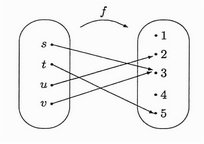
\includegraphics[scale=0.55]{HibCollArrow.jpg}
\end{center}

%---------------------------------------%
\subsection*{Question 6}
%2002 Question 7
Let $\mathcal{S}$ be a set and let $\mathcal{R}$ be a relation on $\mathcal{S}$
Explain what it means to say that $\mathcal{R}$ is

\begin{itemize}
	\item[(i)] reflexive
	\item[(ii)] symmetrix
	\item[(iii)] anti-symmetric
	\item[(iv)] Transitive
\end{itemize}


\subsection*{Question 10}

(a) Given the following adjacency matrices A and B where
%A =
%
%1 0 1
%0 1 2
%1 2 0
%
% ,B =
%
%1 2 0
%2 0 1
%0 1 1

%MAKE NO

%--------------------------------------------%

(i) Say whether or not the graphs they represent are isomorphic.
(ii) Calculate A2 and A4 and say what information each gives about the graph
corresponding to A. [6]
(b) (i) Write down the augmented matrix for the following system of equations.

\[2x + y - z = 2\]
\[x - y + z = 4\]
\[x + 2y + 2z = 10\]
(ii) Use Gaussian elimination to solve the system. [4]

\end{document}

\end{document}

